\documentclass[11pt,a4paper]{article}

\usepackage[utf8]{inputenc}
\usepackage[T1]{fontenc}
\usepackage{lmodern}
\usepackage[slovene]{babel}
\usepackage[margin=2.5cm]{geometry}
\usepackage{graphicx}
\usepackage{float}
\usepackage{url}
\usepackage[hidelinks]{hyperref}

\title{Pregled obstoječih rešitev\\[0.3em]
\large Spletna stran za Čebelarstvo Vidovič}
\author{
  Jaka Štraser \and
  Tadej Čuš
}
\date{17.~november 2026}

\begin{document}

\maketitle

\tableofcontents

\section{Uvod}
V skupini izdelujemo spletno stran za Čebelarstvo Vidovič, manjše družinsko čebelarstvo iz Apač pri Lovrencu na Dravskem polju.
Čebelarstvo spletno stran že ima, vendar je zastarela. Proizvodi so opisani le z dolgimi besedili brez slik, kontaktni obrazec izpisuje napake, na telefonu pa se stran slabo prikaže.

Nova stran bo samo predstavitvena, kupovati na njej ne bo mogoče. Predstavila bo čebelarja in čebelarstvo, šest vrst medu, druge čebelje pridelke (matični mleček, cvetni prah, propolis, vosek), vzrejo matic in priznanja, vse s slikami in krajšimi opisi. Telefonska številka bo vedno vidna v glavi strani, na strani Kontakt pa bodo še e-pošta, Facebook in povezava na zemljevid.
Preden smo začeli z načrtovanjem, smo si ogledali tri podobne strani.

\section{Pregled obstoječih rešitev}

\subsection{Medex}
Medex je eno večjih slovenskih podjetij za čebelje izdelke (med, matični mleček, propolis) in prehranska dopolnila. Čebelje izdelke prodaja od leta 1954.
Na spletni strani~\cite{medex} imajo veliko spletno trgovino, blog in stran o zgodovini podjetja.

Na strani najdemo:
\begin{itemize}
  \item iskalnik izdelkov in spustni meni \emph{Vsi izdelki} s kategorijami,
  \item seznam najbolj prodajanih izdelkov z gumbom \emph{Dodaj v košarico},
  \item akcijske cene skupaj z najnižjo ceno v zadnjih 30 dneh,
  \item prijavo v uporabniški račun in košarico,
  \item blog \#medexlife in stran \emph{Naša zgodba}.
\end{itemize}

Navigacija je pregledna in iskalnik hiter. Cene in popusti so jasno označeni, izdelek pa v košarico dodaš z enim klikom.

Stran je narejena predvsem za prehranska dopolnila, navaden med je bolj v ozadju. Akcijskih pasic je veliko, kupec pa ima občutek, da kupuje pri velikem podjetju in ne pri čebelarju.

\begin{figure}[H]
  \centering
  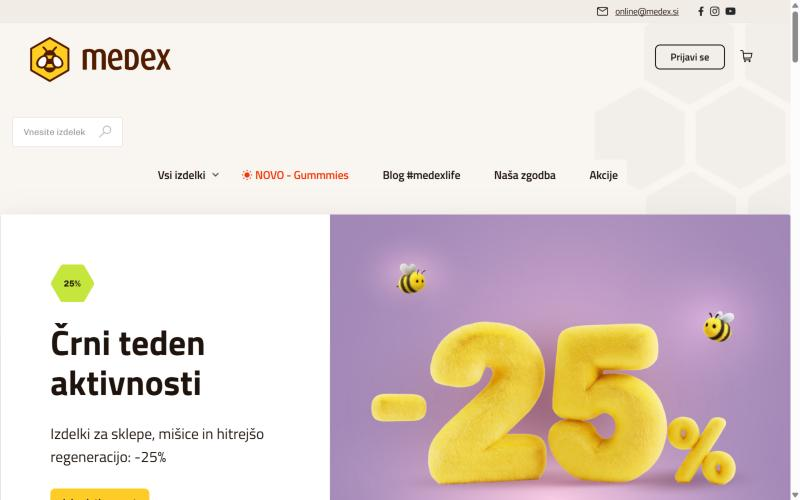
\includegraphics[width=0.9\textwidth]{posnetek-medex.png}
  \caption{Domača stran Medex z iskalnikom, glavnim menijem in akcijsko pasico~\cite{medex}.}
  \label{fig:medex}
\end{figure}

\subsection{Sedanja stran Čebelarstva Vidovič}
Čebelarstvo Vidovič vodi Jože Vidovič, ki samostojno čebelari od leta 2014.
Njegova sedanja stran~\cite{vidovic} je predstavitvena. Opisuje čebelarja, čebelje pridelke in delo čebelarstva.

Na strani najdemo:
\begin{itemize}
  \item naslovno sliko z drsnikom in pozdravno besedilo,
  \item meni z razdelki \emph{O nas}, \emph{Proizvodi} (med, matični mleček, cvetni prah, propolis, vosek), \emph{Aktivnosti}, \emph{Povezave}, \emph{Matice} in \emph{Kontakt},
  \item iskalnik in povezavo na Facebook,
  \item kontaktne podatke in kontaktni obrazec.
\end{itemize}

Na strani \emph{O nas} čebelar sam pripoveduje, kako je začel čebelariti. Pri vsakem pridelku je daljši poučen opis, kontaktni podatki pa so lahko dostopni.

Proizvodi nimajo slik, besedila so dolga in jih je težko preleteti. Videz je zastarel in se ne prilagodi telefonu. Na strani s kontaktnim obrazcem se nad obrazcem izpišejo sistemska opozorila PHP, zaradi katerih je obiskovalec manj prepričan, da obrazec deluje.

\begin{figure}[H]
  \centering
  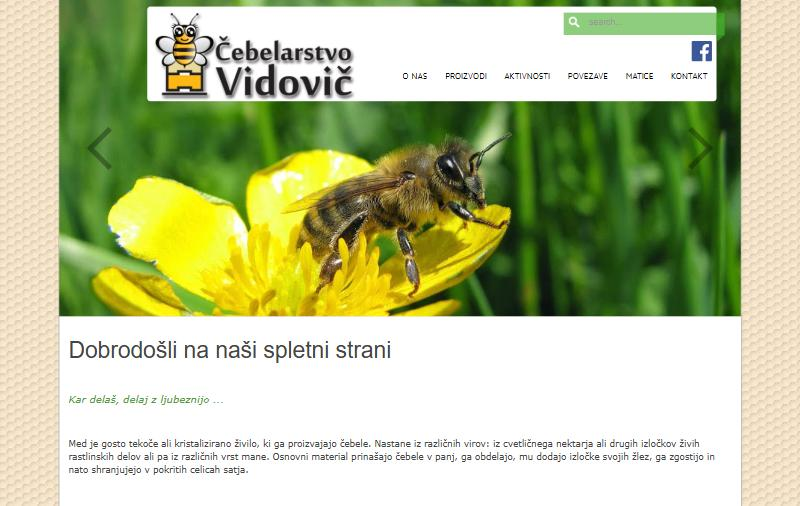
\includegraphics[width=0.9\textwidth]{posnetek-vidovic.png}
  \caption{Sedanja domača stran Čebelarstva Vidovič~\cite{vidovic}.}
  \label{fig:vidovic}
\end{figure}

\subsection{Čebelarstvo Kotnik}
Čebelarstvo Kotnik je družinsko čebelarstvo, ki deluje od leta 1955.
Na spletni strani~\cite{kotnik} prodaja med, izdelke za apiterapijo in poslovna darila, predstavlja pa tudi družino in posestvo.

Na strani najdemo:
\begin{itemize}
  \item spletno trgovino s kategorijami (med po vrstah, apiterapija, darila) in košarico v glavi strani,
  \item gumb \emph{Nakupuj zdaj} na naslovni sliki,
  \item velike povezave \emph{Naša zgodba}, \emph{Naši produkti} in \emph{Posestvo Kotnik} na domači strani,
  \item izpostavljene izdelke s ceno, oceno in oznako \emph{Akcija},
  \item mnenja strank in blog z nasveti.
\end{itemize}

Barve in fotografije se ujemajo z medom. Do trgovine pride kupec z enim klikom, cene in ocene pa vidi že na domači strani. Zaradi mnenj strank nov kupec strani lažje zaupa.

Meni je zelo dolg, ker so v podmenijih našteti skoraj vsi izdelki. Nekaj besedila je ostalo v angleščini (\emph{Your cart}). Zadnja objava na blogu je iz avgusta 2025, prejšnja pa iz leta 2022.

\begin{figure}[H]
  \centering
  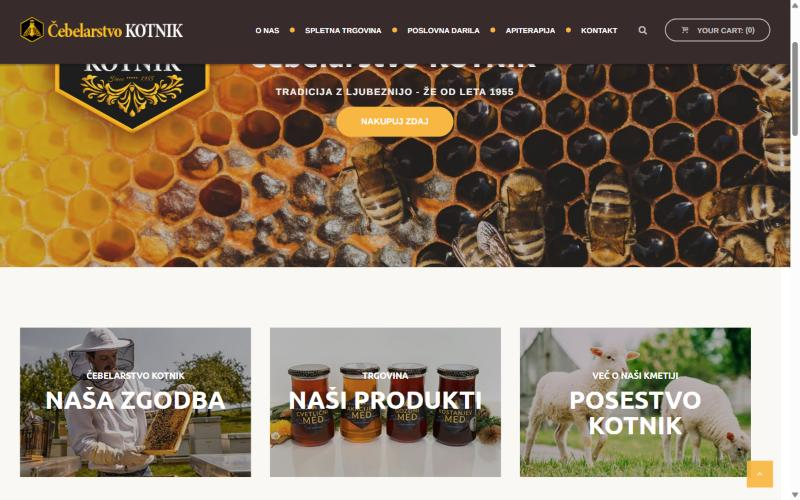
\includegraphics[width=0.9\textwidth]{posnetek-kotnik.png}
  \caption{Domača stran Čebelarstva Kotnik z menijem, košarico in povezavami na glavne razdelke~\cite{kotnik}.}
  \label{fig:kotnik}
\end{figure}

\section{Primerjava}
Tabela~\ref{tab:primerjava} primerja vse tri strani.

\begin{table}[H]
  \centering
  \begin{tabular}{|l|c|c|c|}
    \hline
    \textbf{Funkcionalnost} & \textbf{Medex} & \textbf{Vidovič (sedanja)} & \textbf{Kotnik} \\
    \hline
    Predstavitev čebelarja       & delno & da & da \\
    Proizvodi s slikami          & da    & ne & da \\
    Kontakt na strani            & da    & da (obrazec z napakami) & da \\
    Zgodba čebelarja             & delno & da & da \\
    Blog ali novice              & da    & ne & da \\
    Prilagojeno za telefon       & da    & ne & da \\
    \hline
  \end{tabular}
  \caption{Primerjava pregledanih rešitev.}
  \label{tab:primerjava}
\end{table}

\section{Zaključek}
Od Medexa (slika~\ref{fig:medex}) bomo vzeli pregleden glavni meni in velike fotografije izdelkov.
S sedanje strani Čebelarstva Vidovič (slika~\ref{fig:vidovic}) bomo ohranili čebelarjevo zgodbo, opise čebeljih pridelkov in poseben razdelek o maticah.
Po zgledu Čebelarstva Kotnik (slika~\ref{fig:kotnik}) bomo na domači strani pokazali vse glavne razdelke s fotografijami, ločeno stran pa bo dobila vsaka vrsta medu.

Medex in Kotnik sta spletni trgovini, naša stran pa bo samo predstavitvena, brez košarice, cen in nakupa.
V primerjavi s sedanjo stranjo bodo proizvodi imeli slike in krajše opise, na strani Kontakt ne bo več sistemskih napak, stran pa se bo prilagodila telefonu.
Meni bo krajši kot pri Kotniku: Med, Pridelki, O nas, Priznanja, Kontakt in Matice čebel. Telefonska številka bo vedno v glavi strani, da obiskovalec čebelarja pokliče z enim klikom.
Naslov, telefon in e-pošta bodo vidni na vsaki strani v nogi.

\begin{thebibliography}{9}
  \bibitem{medex} Medex d.o.o., \emph{Medex: Naravna prehranska dopolnila in čebelji izdelki}, \url{https://www.medex.si}, dostop: 17.~11.~2026.
  \bibitem{vidovic} Čebelarstvo Vidovič, \emph{Čebelarstvo Vidovič}, \url{https://www.cebelarstvo-vidovic.si}, dostop: 17.~11.~2026.
  \bibitem{kotnik} Čebelarstvo Kotnik, \emph{Čebelarstvo KOTNIK, že 70 let}, \url{https://cebelarstvo-kotnik.si}, dostop: 17.~11.~2026.
\end{thebibliography}

\end{document}
